%% Supplemental material for "Physics-Exact Credit Assignment for Multi-Agent
%% Flutter Suppression" (submitted to AIAA Journal). Cited from the main
%% text; not subject to the journal's page limit. Reproduces, unabridged,
%% material moved out of the main text solely to meet AIAA's Regular Article
%% length guidance -- every finding stated here is covered by the same seed
%% count and statistical standard noted where it is used in the main text.
\documentclass[11pt]{article}
\usepackage[T1]{fontenc}
\usepackage{lmodern}
\usepackage[letterpaper,margin=1in]{geometry}
\usepackage{amsmath,amssymb,amsthm}
\usepackage{array}
\usepackage{booktabs}
\usepackage{graphicx}
\usepackage{siunitx}
\usepackage{algorithm}
\usepackage{algpseudocode}
\usepackage[hidelinks]{hyperref}
\usepackage[round]{natbib}

\newtheorem{proposition}{Proposition}
\newtheorem{remark}{Remark}

\newcommand{\Uf}{U_{\mathrm{f}}}
% Generated by scripts/fill_numbers.py -- do not edit numeric macros by hand.
\newcommand{\FlutterSpeed}{137.35}
\newcommand{\FeasibleCells}{6}
\newcommand{\TotalCells}{9}
\newcommand{\LocalFbStabilised}{4}
\newcommand{\LocalFbHealthy}{-0.03}
\newcommand{\LqrFixedStabilised}{5}
\newcommand{\LqrFixedHealthy}{-5.15}
\newcommand{\LqrSchedStabilised}{5}
\newcommand{\LqrSchedHealthy}{-5.08}
\newcommand{\LqgLocalStabilised}{5}
\newcommand{\LqgLocalHealthy}{-5.52}
\newcommand{\LqrOracleStabilised}{6}
\newcommand{\LqrOracleHealthy}{-5.07}
\newcommand{\CommOracleStabilised}{6}
\newcommand{\CommOracleHealthy}{-0.18}
\newcommand{\IppoPhysicsStabilised}{6}
\newcommand{\IppoPhysicsHealthy}{-0.25}
\newcommand{\MoccaStabilised}{5}
\newcommand{\MoccaHealthy}{-0.14}
\newcommand{\RecurrentOnlyStabilised}{5}
\newcommand{\RecurrentOnlyHealthy}{-0.04}
\newcommand{\BestRobustVariant}{comm\_oracle}
\newcommand{\BestRobustStabilised}{6}
\newcommand{\BestNominalVariant}{ippo\_physics}
\newcommand{\BestNominalHealthy}{-0.25}
\newcommand{\ResultsSummarySentence}{\emph{[ResultsSummarySentence: to be written]}}
\newcommand{\ResultsNarrative}{\emph{[ResultsNarrative: to be written]}}
\newcommand{\ResultsAblations}{\emph{[ResultsAblations: to be written]}}
\newcommand{\PhaseNarrative}{\emph{[PhaseNarrative: to be written]}}
\newcommand{\ConclusionSentence}{\emph{[ConclusionSentence: to be written]}}


\title{Supplemental Material: Physics-Exact Credit Assignment for\\
Multi-Agent Flutter Suppression}
\author{}
\date{}

\begin{document}
\maketitle

\noindent This document collects material referenced from the main text but
moved here to meet the journal's page-length guidance. Section, table, and
figure numbers below are internal to this document (prefixed S) and are
cross-referenced from the main text by name, not by number.

\section*{S1. Network architecture, training procedure, and convergence}
\label{sec:s1}

\subsection*{Network architecture}

Figure~\ref{fig:architecture} shows the full policy pipeline. Every variant
feeds agent $k$'s local observation $o_k^t \in \mathbb{R}^{12}$,
concatenated with a one-hot agent identity and (when enabled) an incoming
consensus message $e_k^t$, through a two-layer $\tanh$ multilayer
perceptron of width 128 to a latent $\ell_k^t$. Parameters are shared
across agents; only the one-hot identity varies, which keeps the parameter
count independent of the number of surfaces and is what makes the
eight-surface scaling probe (Section~S5) possible without retraining a
wider network.

\begin{figure}[h]
\centering
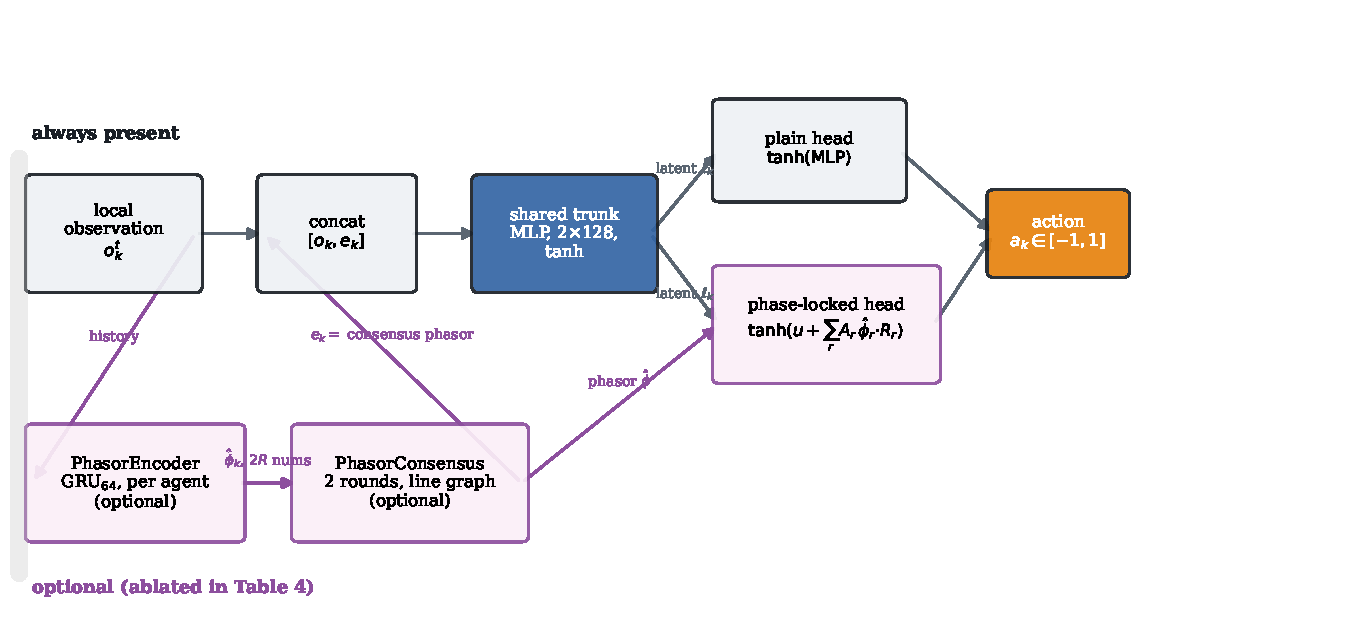
\includegraphics[width=0.92\textwidth]{figures/fig_architecture.pdf}
\caption{The policy network. Grey boxes and the plain head are present in
every variant; the pink boxes and the phase-locked head are the mechanisms
ablated in the main text's architecture table, so \texttt{recurrent\_only}
keeps the encoder but not consensus or the head, \texttt{mocca\_nohead}
keeps the encoder and consensus but ends in the plain head, and
\texttt{mocca} is the full diagram.}
\label{fig:architecture}
\end{figure}

\paragraph{Phasor encoder (\texttt{recurrent\_only} and beyond)}
A single instantaneous accelerometer reading cannot distinguish a mode
moving up from the same displacement moving down, so recovering phase
needs memory. A per-agent GRU cell \citep{hausknecht2015drqn} carries a
hidden state $h_k^t \in \mathbb{R}^{64}$ across the episode:
\begin{equation}
h_k^t = \mathrm{GRU}\!\left(o_k^t, h_k^{t-1}\right), \qquad
\hat\phi_k^t = \tanh\!\left(W_{\mathrm{out}}\, h_k^t\right) \in \mathbb{R}^{4},
\label{eq:encoder}
\end{equation}
read as two pairs $(\hat\phi_{k,r}^{\cos}, \hat\phi_{k,r}^{\sin})$, one per
retained mode. The output is passed through $\tanh$ before use anywhere
downstream: an unbounded phasor multiplied by a gain inside the action head
saturates that head's own $\tanh$ at initialisation and kills the gradient
before training starts, which is what the first implementation of this
policy did. The phasor is carried as a $(\cos,\sin)$ pair rather than an
angle throughout, so wrap-around is not a discontinuity the network has to
fight.

\paragraph{Phasor consensus (\texttt{mocca} and \texttt{comm\_raw})}
The communication mechanism is $T{=}2$ rounds of averaging over the
spanwise line graph -- agent $k$ exchanges only with agents $k{-}1$ and
$k{+}1$, what a distributed avionics bus physically offers. The operator
\begin{equation}
P = (1-w)\,I + w\,A, \qquad w = 0.5,
\label{eq:consensus-operator}
\end{equation}
with $A$ the row-normalised adjacency of the line graph, is fixed rather
than learned, so consensus adds no parameters; the bandwidth cost is the
message itself, 4 numbers per agent per round regardless of surface count.
The consensus message is $e^t = P^T \hat\phi^t$, read back into the trunk
of each agent as $e_k^t$. \texttt{comm\_raw} replaces $\hat\phi_k^t$ in this
pipeline with the agent's raw local observation instead of the encoder's
phasor estimate, testing whether the phasor abstraction itself does
anything relative to simply broadcasting what a neighbour sees.

\paragraph{Phase-locked action head (the full \texttt{mocca} architecture)}
For retained mode $r$ with consensus phasor $(\hat\phi_r^{\cos},
\hat\phi_r^{\sin})$, the head emits a gain $A_r \in [-1,1]$ and a phase
offset via a unit vector $(\cos\psi_r, \sin\psi_r)$, and acts by rotating
the phasor:
\begin{equation}
\rho_r = \hat\phi_r^{\cos}\cos\psi_r - \hat\phi_r^{\sin}\sin\psi_r, \qquad
a_k = \tanh\!\left(u + \sum_{r} A_r\, \rho_r\right),
\label{eq:phaselocked}
\end{equation}
where $u$ is an additional broadband channel from the same latent. The
resonant term is \emph{added} to $u$ rather than replacing it, a strict
generalisation of the plain head: setting every $A_r$ to zero recovers an
unconstrained policy exactly. An earlier version of this head replaced $u$
instead of adding to it, turning a resonant prior into a restriction, and
scored worse than removing the head entirely -- \texttt{mocca\_nohead} is
the trunk and consensus without this head, i.e.\ the plain
$\tanh(\mathrm{MLP})$ output at the top of Figure~\ref{fig:architecture}.

\paragraph{Critic}
The critic is a separate two-layer MLP taking the same per-agent input as
the actor by default; a fully centralised critic (fed the true modal state
instead) was tried and made no measurable difference, consistent with this
being a dense-reward, low-partial-observability credit problem rather than
one where value estimation is the bottleneck. Every head has its final
layer scaled by $0.01$ at initialisation so a fresh policy is close to a
no-op, which is what makes the residual variants well-posed from the first
update rather than starting by fighting the base controller.

\subsection*{Training procedure}

We use shared-parameter multi-agent PPO \citep{schulman2017ppo,yu2022mappo}
with generalised advantage estimation \citep{schulman2016gae} and per-agent
advantages, since each agent receives a different reward. Updates run on
sequences: minibatches are segments of consecutive steps unrolled with
gradient from a detached stored hidden state. Sampling shuffled individual
timesteps, as we did initially, trains any recurrence as a one-step map and
gives a recurrent encoder no temporal gradient at all
\citep{hausknecht2015drqn}. Algorithm~\ref{alg:mocca} summarises the
procedure.

\begin{algorithm}[h]
\caption{Training with the blended (exact-plus-shaping) credit}
\label{alg:mocca}
\begin{algorithmic}[1]
\State Assemble $M,C,K,L,B$ at the sampled airspeed; small-gain init of the
action head
\For{each update}
  \State Ease the task distribution by the curriculum fraction
  \For{$t=1,\dots,T$}
    \State Each agent $k$ acts on its own $o_k^t$; step the coupled plant and
    actuators
    \State $P_k^t \gets (\dot q^\top b_k)\,\delta_k^t$
    \Comment{closed form}
    \State $r_k^t \gets -P_k^t/(E^t+\varepsilon)
      + w\,[\Phi^{t+1}-\Phi^{t}]/\Delta t$
    \Comment{$\Phi=-\log\frac{E+\varepsilon}{E_{\mathrm{ref}}}$}
  \EndFor
  \State Compute per-agent GAE advantages
  \For{each epoch, each minibatch of \emph{sequences}}
    \State Unroll $L_{\mathrm{bptt}}$ steps from a detached hidden state; zero it
    where an episode ended
    \State PPO clipped objective $+$ value loss $-$ entropy bonus
  \EndFor
\EndFor
\end{algorithmic}
\end{algorithm}

\subsection*{Hyperparameters}

Table~\ref{tab:params-ppo} lists the PPO and network hyperparameters
shared across every learned variant, except where a hyperparameter is
itself the subject of an ablation (the initial exploration standard
deviation, and the presence or absence of the architectural mechanisms
above).

\begin{table}[h]
\centering
\caption{PPO and network hyperparameters.}
\label{tab:params-ppo}
\begin{tabular}{@{}lp{5.6cm}@{}}
\toprule
Hyperparameter & Value \\
\midrule
Parallel environments & 128 \\
Rollout length & 128 steps \\
Epochs per update & 4 \\
Minibatches per epoch & 4 \\
BPTT segment length & 32 steps \\
Learning rate (Adam) & $3\times 10^{-4}$ \\
Discount $\gamma$ & 0.995 \\
GAE $\lambda$ & 0.95 \\
PPO clip range & 0.2 \\
Value loss coefficient & 0.5 \\
Entropy coefficient & $2\times 10^{-3}$ (0 in the exploration sweep) \\
Max gradient norm & 0.5 \\
Curriculum fraction & 0.4 of training \\
Hidden layer width (trunk) & 128 \\
Phasor encoder hidden width & 64 \\
Retained modes per phasor & 2 \\
Consensus rounds & 2 \\
Action-head output-layer gain (init.) & 0.01 \\
\bottomrule
\end{tabular}
\end{table}

\subsection*{Compute and reproducibility}

Every learned variant trains for $1.5{\times}10^6$ environment steps
across 128 vectorised environments on a single NVIDIA RTX 5000 Ada
(laptop) GPU, using PyTorch 2.6. Across the 86 training runs behind the
main results and ablations, median wall-clock training time is
\SI{331}{\second} (minimum \SI{246}{\second} for a plain policy, maximum
\SI{1115}{\second} for the full \texttt{mocca} architecture, whose GRU
encoder and consensus rounds are the most expensive forward pass in the
ablation set), at a median throughput of $4.5{\times}10^3$ environment
steps per second -- the batched environment rather than the network is the
bottleneck at this scale. The full set of runs reported in this paper --
the credit and architecture ablations, the eight-surface scaling probe,
and every additional probe in Section~S5 -- totals \SI{12.7}{\hour} of GPU
time; no result in this paper required infrastructure beyond a single
workstation GPU.

\subsection*{Training convergence}

Figure~\ref{fig:learning} gives the training-time behaviour behind every
learned number in the main text: mean structural energy and divergence
rate over training on the curriculum task distribution, averaged across
seeds. Every variant is within a small margin of its asymptote by
\num{750000} of the \num{1500000} environment steps budgeted, confirming
the training budget was chosen with headroom rather than tuned to
convergence after the fact. \texttt{residual\_only} starts substantially
lower than every other variant and stays there for the first
\num{200000} steps, the training-time signature of the small-gain
initialisation: it inherits the decentralised LQG base law's performance
from update one rather than the near-open-loop performance every other
variant starts from. The divergence rate -- a training statistic, not the
evaluation metric of the main text's results table -- spikes above
\SI{0.5}{\percent} only in the first few thousand steps, before any policy
has learned anything and while the curriculum is still easing in, and
settles below \SI{0.15}{\percent} thereafter for every variant: the
curriculum keeps training itself stable even where the resulting policy
later struggles on the harder end of the evaluation grid.

\begin{figure}[h]
\centering
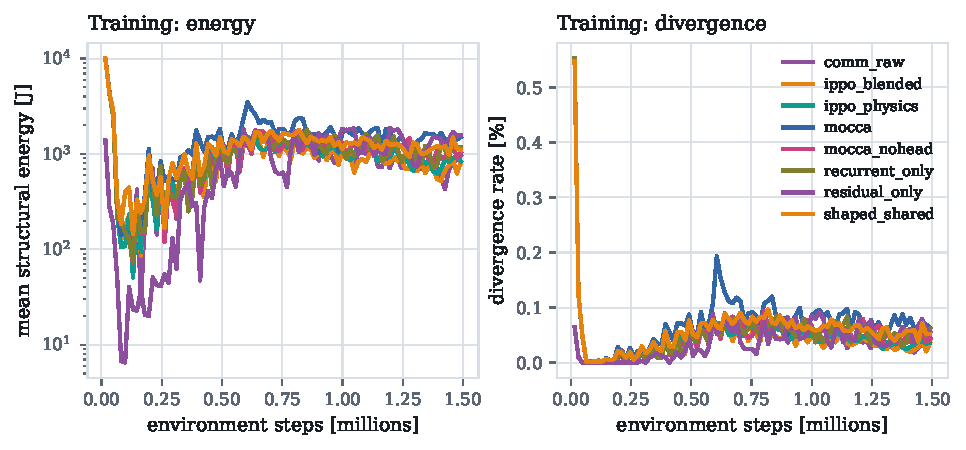
\includegraphics[width=\textwidth]{figures/fig_learning.pdf}
\caption{Training-time mean structural energy (left, log scale) and
divergence rate (right) against environment steps, averaged over seeds,
for every credit and architecture variant. All variants reach a stable
plateau well inside the training budget; \texttt{residual\_only} converges
fastest because it starts from a decentralised LQG base law rather than
from scratch.}
\label{fig:learning}
\end{figure}

\section*{S2. Baseline controller synthesis}
\label{sec:s2}

This section gives the synthesis equations behind every rung of the
classical baseline ladder in the main text, so that ``discrete-time LQG on
local accelerometers'' is reproducible from this document alone.

\subsection*{Augmented, discretised plant}

Actuator lag is part of the design plant, not an unmodelled disturbance
added afterwards: with $z=[q,\dot q, x_{\mathrm{w}}, \delta]$ (the state of
the equation of motion augmented with the deflections) and first-order
servo lag of time constant $\tau_k$ per surface,
\begin{equation}
\dot z = \tilde A z + \tilde B u, \qquad
\tilde A = \begin{bmatrix} A & B \\ 0 & -\mathrm{diag}(\tau_k^{-1}) \end{bmatrix},
\quad
\tilde B = \begin{bmatrix} 0 \\ \mathrm{diag}(\tau_k^{-1}) \end{bmatrix},
\label{eq:augplant}
\end{equation}
where $A,B$ are the plant matrices in state-space form and
$u\in[-1,1]^K$ is the normalised command. Every controller in this study is
synthesised in discrete time at the \SI{200}{\hertz} control rate via the exact
zero-order-hold discretisation
\begin{equation}
\begin{bmatrix} \Phi & \Gamma \\ 0 & I \end{bmatrix}
= \exp\!\left( \begin{bmatrix} \tilde A & \tilde B \\ 0 & 0 \end{bmatrix} \Delta t \right),
\label{eq:zoh}
\end{equation}
giving $z_{t+1} = \Phi z_t + \Gamma u_t$. Designing in continuous time and
integrating the resulting gain with a forward-Euler step at $\Delta t=\SI{5}{ms}$
is not a minor approximation here: the wake states have $|\lambda|$ up to
$\sim\!\SI{1.3e4}{\radian\per\second}$, so $\Delta t\,|\lambda|\approx 63$, and
the observer built that way is unstable regardless of how good its gain is.

\subsection*{LQR gain}

The state cost weights physical structural energy rather than an arbitrary
diagonal, plus a light penalty on held deflection so the optimum does not park
surfaces at the travel limit:
\begin{equation}
Q = \begin{bmatrix} K_{\mathrm{modal}} & & \\ & M_{\mathrm{modal}} & \\ & & \mathrm{diag}\!\left(w_{\mathrm{rate}}/\delta_{\max,k}^2\right) \end{bmatrix},
\qquad
R = \mathrm{diag}\!\left(w_{\mathrm{effort}}/\delta_{\max,k}^2\right),
\label{eq:lqrcost}
\end{equation}
with $w_{\mathrm{effort}}=2{\times}10^4$, $w_{\mathrm{rate}}=10^2$ throughout.
The discrete-time algebraic Riccati equation
\begin{equation}
P = \Phi^{\!\top} P \Phi - \Phi^{\!\top} P \Gamma \left(R+\Gamma^{\!\top} P \Gamma\right)^{-1} \Gamma^{\!\top} P \Phi + Q
\label{eq:dare}
\end{equation}
gives the gain $\mathcal{K}=(R+\Gamma^{\!\top} P \Gamma)^{-1}\Gamma^{\!\top} P \Phi$
and command $u_t=-\mathcal{K} z_t$ \citep{anderson2007optimal}.
\texttt{BatchedLQR} solves \eqref{eq:dare} once at a fixed design speed;
\texttt{BatchedScheduledLQR} solves it on a 9-point airspeed grid over
the evaluation envelope and linearly interpolates $\mathcal{K}$ between grid
points; \texttt{BatchedJamAwareLQR} additionally zeros the failed surface's
column of $\Gamma$ per failure hypothesis and resolves \eqref{eq:dare} for each
hypothesis on the same grid, so the surviving surfaces' gains already account
for the loss rather than compensating for it reactively.

\subsection*{Local rate feedback}

The floor of the ladder uses no plant model: with $\dot h_k,\dot\alpha_k$ the
locally sensed plunge and twist rate at surface $k$'s own station,
\begin{equation}
u_k = -\left(g_h\,\dot h_k + g_\alpha\,\dot\alpha_k\right), \qquad g_h=0.35,\ g_\alpha=0.9,
\label{eq:ratefeedback}
\end{equation}
clipped to $[-1,1]$.

\subsection*{Steady-state Kalman observer on local accelerometers}

The centralised and decentralised LQG rungs replace the true state $z_t$ in
$u_t=-\mathcal{K}\hat z_t$ with an estimate driven only by the accelerometer
channels the agents themselves observe, $y_t = H z_t$, where $H$ is built from
the acceleration rows of the plant rather than a selection matrix, since an
accelerometer measures $\ddot q$, an algebraic function of the state rather
than a state itself. The steady-state predictor-form filter is
\begin{align}
\Sigma &= \Phi\Sigma\Phi^{\!\top} + W
- \Phi\Sigma H^{\!\top}\!\left(H\Sigma H^{\!\top}+V\right)^{-1}\! H\Sigma\Phi^{\!\top},
\label{eq:kalmanriccati} \\
L &= \Phi\Sigma H^{\!\top}\!\left(H\Sigma H^{\!\top}+V\right)^{-1}, \\
\hat z_{t+1} &= \Phi\hat z_t + \Gamma u_t + L\left(y_t - H\hat z_t\right),
\label{eq:kalmanupdate}
\end{align}
with process noise $W=10^{-4}I$ and measurement noise
$V=10^{-6}\,\mathrm{diag}(\lVert H_i\rVert^2)$ scaled per-channel, since
accelerometer rows of $H$ have norms of order $10^4$--$10^5$ and an unscaled
$V$ demands impossible measurement precision and drives $L$ to blow up
\citep{anderson2007optimal}. \texttt{BatchedLQG} solves
\eqref{eq:kalmanriccati}--\eqref{eq:kalmanupdate} once with $H$ built from all
six channels and $\mathcal{K}$ commanding all three surfaces jointly, on the
same speed grid as the scheduled LQR. \texttt{Batched\-Decentralized\-LQG}
solves an \emph{independent} instance of
\eqref{eq:kalmanriccati}--\eqref{eq:kalmanupdate} per surface $k$, with $H$
restricted to $k$'s own two accelerometer rows and $\Gamma$ restricted to $k$'s
own column, so agent $k$'s estimate, gain and command never depend on any
other surface's measurement or actuation -- the discrete-time, model-based
analogue of the information structure the learned policies are given. Its
scheduling grid spans the same $[1.0,1.5]\,\Uf$ range as the training
curriculum exactly, by construction rather than coincidence, so the
comparison in the main text is not confounded by the classical design being
scheduled over a narrower envelope than the learned policy was trained on.

\subsection*{Re-tuning the decentralised LQG for control-authority margin}

\texttt{BatchedRobustDecentralizedLQG} is structurally identical to
\texttt{BatchedDecentralizedLQG}: same per-surface observer, same
restriction to each agent's own two accelerometers and own actuator. Two
remedies for its lack of a guaranteed margin \citep{doyle1978guaranteed}
were checked. The first, loop transfer recovery \citep{doylestein1981ltr},
boosts the process-noise weighting $W$ in \eqref{eq:kalmanriccati} by
$\rho\, b_k b_k^{\top}$ (agent $k$'s own reduced input column) as
$\rho\to\infty$, pushing the filter loop toward the full-state loop shape.
Sweeping $\rho$ from $0$ to $10^4$ changes the control-authority margin
(the largest reduction in true control authority, relative to the design
assumption, the closed loop remains stable under, found by bisection on
the discrete-time closed-loop spectral radius) not at all: it stays at
$0.158$ at $1.45\,\Uf$ throughout. Comparing against the same gain applied
with perfect (observer-free) state feedback, whose margin is also $0.158$,
shows why: the observer is not the bottleneck, so there is nothing for an
observer-side remedy to recover.

The second remedy, and the one \texttt{BatchedRobustDecentralizedLQG}
actually uses, re-weights the LQR cost \eqref{eq:lqrcost} itself:
$w_{\mathrm{effort}}$ increased from $2\times10^4$ to $10^6$, with
$w_{\mathrm{rate}}$, $W$ and $V$ unchanged. This raises the
control-authority margin from $0.158$ to $0.179$ before plateauing (no
further gain to $w_{\mathrm{effort}}=10^{7}$), at a cost to nominal decay
rate: the closed-loop growth rate at design conditions worsens from
$0.9744$ to $0.9916$ in discrete-time terms.
\texttt{scripts/robust\_baseline\_check.py} reproduces both checks.

\section*{S3. Plant model supplementary material}
\label{sec:s3}

\subsection*{Testbed parameters}

Table~\ref{tab:params-wing} gives the geometric and structural parameters
of the wing and Table~\ref{tab:params-actuator} the actuator and sensing
parameters, common to every controller in this study.

\begin{table}[h]
\centering
\caption{Wing geometry and structural properties.}
\label{tab:params-wing}
\begin{tabular}{lr}
\toprule
Parameter & Value \\
\midrule
Semispan & \SI{6.096}{\metre} \\
Chord & \SI{1.8288}{\metre} \\
Mass per unit length & \SI{35.71}{\kilo\gram\per\metre} \\
Polar inertia per unit length (about EA) & \SI{8.64}{\kilo\gram\metre} \\
Bending stiffness $EI$ & $\SI{9.77e6}{\newton\metre\squared}$ \\
Torsional stiffness $GJ$ & $\SI{0.987e6}{\newton\metre\squared}$ \\
Elastic axis & \SI{33}{\percent} chord \\
Centre of gravity & \SI{43}{\percent} chord \\
Bending / torsion modes retained & 2 / 2 \\
Aerodynamic strips & 24 \\
Air density (sea level) & \SI{1.225}{\kilo\gram\per\cubic\metre} \\
\bottomrule
\end{tabular}
\end{table}

\begin{table}[h]
\centering
\caption{Control surface, actuator and sensing parameters (identical for all
three surfaces).}
\label{tab:params-actuator}
\begin{tabular}{@{}lp{6.0cm}@{}}
\toprule
Parameter & Value \\
\midrule
Spanwise bands (fraction of semispan) & $[0.05,0.40]$, $[0.40,0.72]$, $[0.72,0.98]$ \\
Hinge location & \SI{75}{\percent} chord \\
Deflection travel & $\pm\SI{15}{\degree}$ \\
Rate limit & \SI{200}{\degree\per\second} \\
Actuator time constant & \SI{20}{\milli\second} \\
Control update rate & \SI{200}{\hertz} \\
Local observation per agent & 2 accelerometers, plunge/twist rate, own
saturation, air data \\
\bottomrule
\end{tabular}
\end{table}

\subsection*{What flutter and its suppression look like}

Every quantity in the main text is a scalar derived from a wing that is
physically bending and twisting, worth seeing once before reducing it to
decay rates. Figure~\ref{fig:filmstrip} gives the same initial
\SI{5}{\centi\metre} tip pluck under two treatments at $U/\Uf=1.10$, six
shared instants apart, on one shared deformation scale. The top row is
what ``flutter'' names: bending and torsion lock into a fixed phase
relationship and the response grows visibly within under a second, until
the linear model is no longer valid. The bottom row is the identical pluck
under centralised LQR: by the second frame the deflection is already
smaller than at $t=0$, and stays there. Both are literal rollouts of the
plant at the flight condition used throughout the main text's results
section. A supplementary animation of all four classical cases (open loop,
centralised LQR, local rate feedback, and centralised LQR with the
outboard surface jammed) is provided alongside the code.

\begin{figure}[h]
\centering
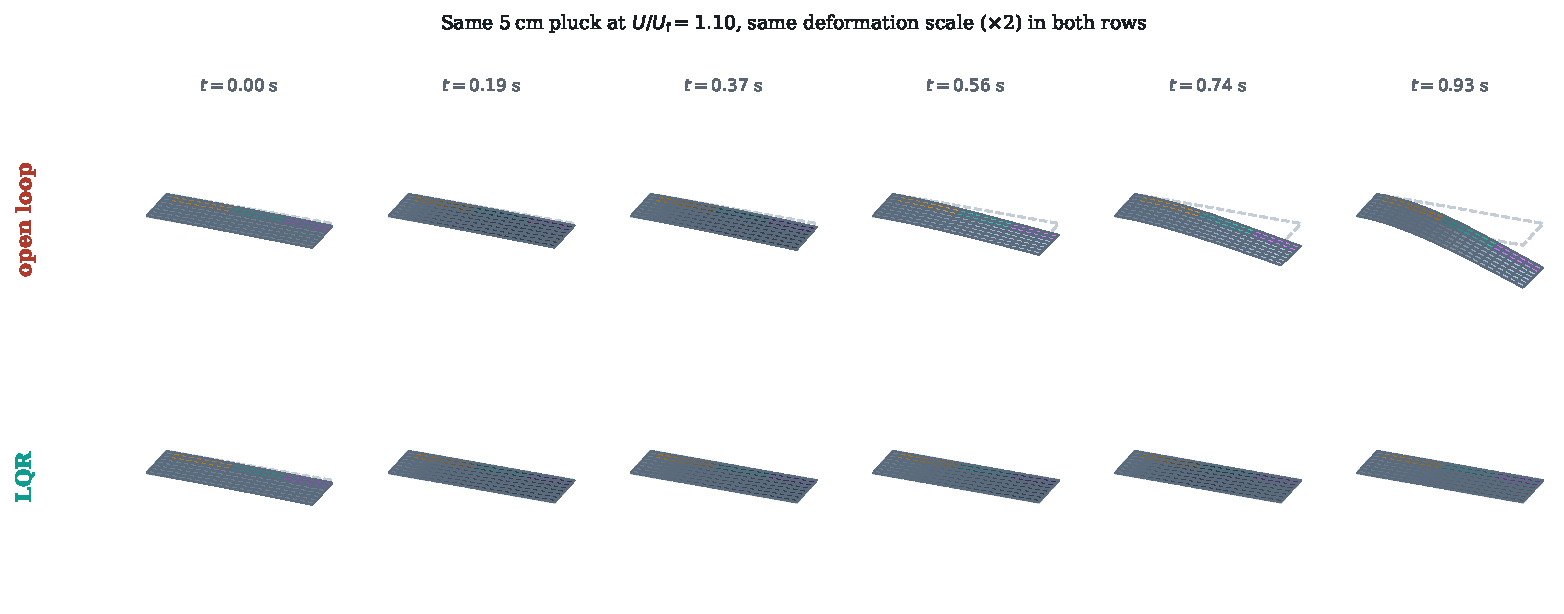
\includegraphics[width=\textwidth]{figures/fig_filmstrip.pdf}
\caption{Six shared instants of the same \SI{5}{\centi\metre} initial tip
pluck at $U/\Uf=1.10$, one shared deformation scale (dashed outline: the
undeformed reference planform). Top: open loop -- bending and torsion
coalesce and the response diverges within \SI{0.93}{\second}, at which
point it leaves the linear regime and the rollout is stopped. Bottom: the
identical pluck under centralised LQR, suppressed by the second frame and
held near zero afterward.}
\label{fig:filmstrip}
\end{figure}

\begin{figure}[h]
\centering
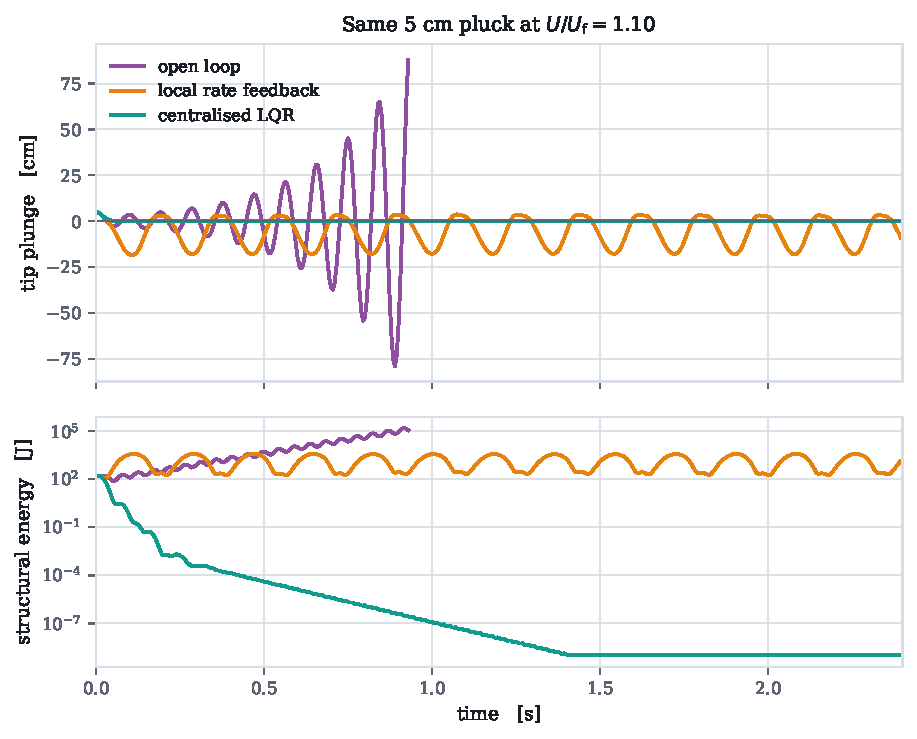
\includegraphics[width=0.82\textwidth]{figures/fig_timedomain.pdf}
\caption{Tip plunge (top) and structural energy (bottom, log scale) for
the same initial pluck under three of the five classical rungs. Local rate
feedback neither grows nor decays: it damps local motion but never engages
the unstable mode.}
\label{fig:timedomain}
\end{figure}

\begin{figure}[h]
\centering
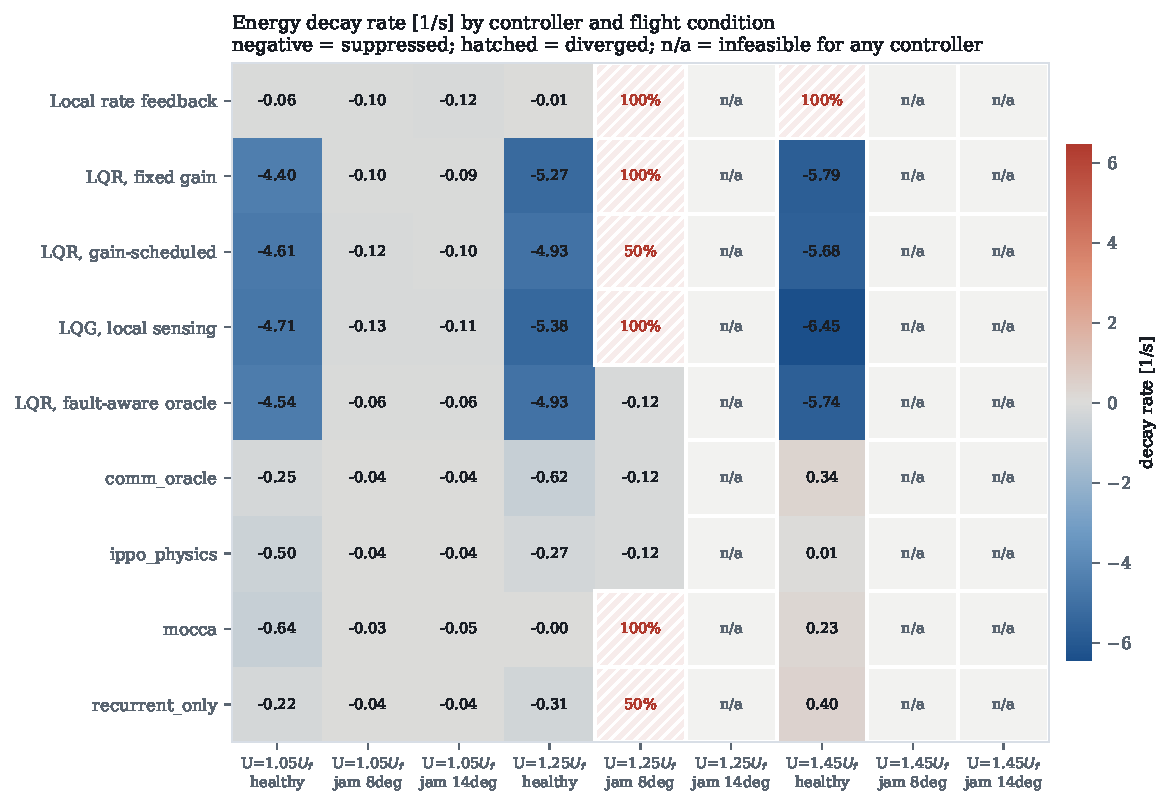
\includegraphics[width=\textwidth]{figures/fig_comparison.pdf}
\caption{Decay rate by controller and condition. Hatching marks
divergence. The same data as the main text's results table, shown
graphically.}
\label{fig:comparison}
\end{figure}

\begin{figure}[h]
\centering
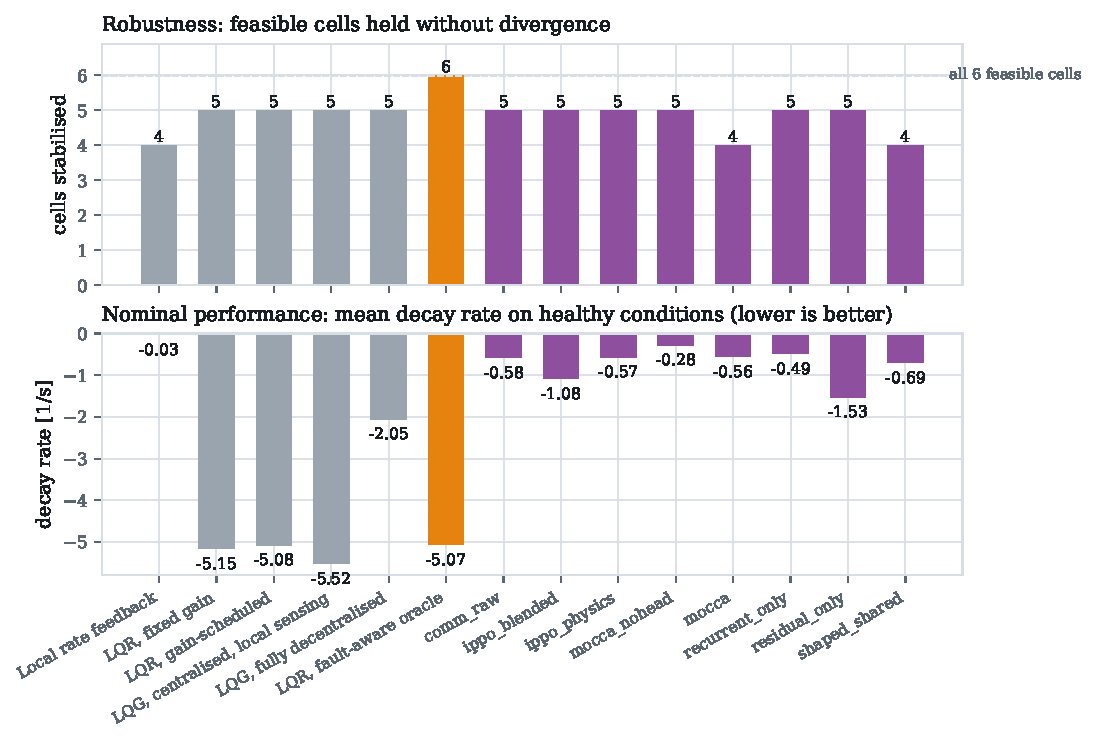
\includegraphics[width=\textwidth]{figures/fig_ablation.pdf}
\caption{Every controller and variant on one axis. Top: feasible
conditions held without divergence, out of the six the fault-aware oracle
shows are stabilisable. Bottom: mean decay rate on healthy conditions. The
learned variants (purple) match the classical rungs on robustness while
trailing them on nominal damping, except for \texttt{residual\_only},
which is the strongest learned result on both axes simultaneously.}
\label{fig:ablation}
\end{figure}

\subsection*{Cross-validation against an unsteady vortex-lattice solver}

The model buys speed with two approximations a reader is entitled to
distrust: two-dimensional strip aerodynamics, and quasi-steady flap
derivatives that neglect the flap's own shed wake. We quantified both
against SHARPy \citep{delcarre2019sharpy}, which couples an unsteady
vortex-lattice method \citep{murua2012uvlm} to a geometrically exact beam.
The comparison is clean because SHARPy's own Goland template carries
structural data identical to ours, so any disagreement is about the
aerodynamics.

\paragraph{Flutter point} SHARPy places flutter at
\SI{154.46}{\metre\per\second} and \SI{69.3}{\radian\per\second} at sea
level, against \SI{137.35}{\metre\per\second} and
\SI{69.34}{\radian\per\second} for our model. The \emph{frequency} agrees
to \SI{0.06}{\percent}, so both identify the same bending--torsion
coalescence; the critical speed differs by \SI{-11.1}{\percent}. That
direction is what two-dimensional aerodynamics predicts, since strip
theory has no tip relief, over-predicts loading near the tip, and
therefore under-predicts the flutter speed. Our plant is conservative,
the safe direction for a control study.

\paragraph{Control authority} This discrepancy runs the other way and is
larger. A part-span flap loses effectiveness to spanwise carryover and to
flow around its ends, neither of which a sectional derivative represents.
Integrating our thin-airfoil $C_{l\delta}=3.826$ per radian over the
flapped span (\SI{25}{\percent} of span, read from the generated
aerodynamic grid) gives a whole-wing $\mathrm{d}C_L/\mathrm{d}\delta$ of
$0.957$ per radian, against $0.495$ from UVLM. Our plant over-estimates
control authority by a factor of $1.9$, grid-converged to within
\SI{3}{\percent} between $8{\times}16$ and $16{\times}32$ panels.

\paragraph{Consequence} Every controller in this study, classical and
learned, was evaluated on the same plant and received the same inflated
authority, so relative comparisons, ablations and significance tests are
unaffected. Absolute decay rates would not transfer unchanged to a UVLM
plant, and we do not claim they would. The two discrepancies act in
opposite directions -- a harder flutter problem, an easier control problem
-- so they cannot be combined into a single safety factor.

\section*{S4. Related-work positioning}
\label{sec:s4}

Table~\ref{tab:positioning} summarises this paper against the literature
it draws on, since no single prior study we are aware of combines more
than one of these axes: multi-agent treatment of the individual control
surfaces of one wing, a credit signal derived in closed form from the
plant's own physics rather than estimated, and validation of the plant
itself against a higher-fidelity solver rather than only against a
published linear benchmark.

\begin{table}[h]
\centering
\caption{This paper against the literature it draws on. A \checkmark
marks that the property holds for the representative citation(s) in that
row; \texttt{--} marks that it does not; \texttt{n/a} marks that the axis
does not apply to that line of work at all (a single-agent or
single-regulator method has no multi-agent credit decomposition to be
closed-form \emph{or} estimated, so neither \checkmark nor \texttt{--}
would be meaningful there).}
\label{tab:positioning}
\small
\begin{tabular}{@{}p{4.4cm}ccc@{}}
\toprule
& Multi-agent & Closed-form & Validated against \\
& surfaces & credit & higher-fidelity solver \\
\midrule
Classical AFS \citep{karpel1982design,waszak2001robust} & -- & n/a & varies \\
Adaptive AFS \citep{downs2023adaptive,mozaffarijovin2024l1} & -- & n/a & -- \\
Learned AFS \citep{stallflutter2025,circulation2023,flyingwing2022} & -- & -- & -- \\
General MARL credit \citep{sunehag2018vdn,rashid2018qmix,foerster2018coma} & \checkmark & -- & n/a \\
Residual control \citep{johannink2019residual,silver2018residual} & -- & -- & n/a \\
This paper & \checkmark & \checkmark & \checkmark \\
\bottomrule
\end{tabular}
\end{table}

\section*{S5. Additional probes}
\label{sec:s5}

The results in the main text are held to a fixed standard: six seeds,
Welch's $t$-test, Cohen's $d$ and Hedges' $g$, Holm-Bonferroni corrected.
Several further questions arose directly out of those results and were
checked, but not all to the same standard; they are reported here as
probes rather than findings.

\paragraph{Exploration-scale variance at six seeds versus two}
An initial two-seed pilot of the spread behind the plateau discussed in
the main text's exploration-scale section suggested it fell sharply
between the conventional and matched scale ($0.132$ at $\sigma=0.30$ to
$0.016$ at $\sigma=0.05$); the six-seed measurement reported in the main
text does not confirm that ($0.325$ at $\sigma=0.30$ to $0.257$ at
$\sigma=0.05$), a second instance in this study of a two-seed spread
understating the true variance, alongside the credit-versus-shaping
correction in the credit-assignment ablation. The interior optimum and the
factor-of-two effect on the mean are what survive at six seeds; the claim
that the spread itself shrinks sharply at the matched scale does not, and
the main text does not make it.

\paragraph{Eight-surface scaling}
Section~V of the main text reports that all nine evaluation conditions
become feasible for the learned policies at eight surfaces. Table~\ref{tab:probes}
gives the numbers behind that sentence, one or two seeds each at
$\sigma=0.05$; every healthy-decay value is listed per seed, not averaged,
because two points do not estimate a standard deviation.

\begin{table}[h]
\centering
\caption{Additional probes, one or two seeds each, at $\sigma=0.05$.
\texttt{-{}-} marks a probe not run for that variant.}
\label{tab:probes}
\small
\begin{tabular}{@{}>{\raggedright\arraybackslash}p{3.6cm}l>{\raggedright\arraybackslash}p{3.4cm}c@{}}
\toprule
Probe & Variant & Healthy decay [1/s], per seed & Held \\
\midrule
\multicolumn{4}{@{}p{0.97\linewidth}@{}}{\emph{Do the negative mechanisms of the architecture ablation also hurt as a residual correction?}} \\
residual + raw comm. & \texttt{residual\_comm} & $-0.697,\ -0.247$ & 6/9, 6/9 \\
residual + health-channel consensus & \texttt{residual\_health} & $-0.518,\ -0.066$ & 5/9, 5/9 \\
\addlinespace
\multicolumn{4}{@{}p{0.97\linewidth}@{}}{\emph{Does supervising the encoder on the true modal phasor help?}} \\
supervised encoder, plain head & \texttt{aux\_encoder} & $-0.219,\ -0.029$ & 5/9, 5/9 \\
supervised encoder, residual & \texttt{aux\_residual} & $-0.431,\ -0.510$ & 5/9, 5/9 \\
\addlinespace
\multicolumn{4}{@{}p{0.97\linewidth}@{}}{\emph{Eight-surface scaling}} \\
consensus, plain head, $N{=}8$ & \texttt{mocca\_nohead} & $-0.028,\ -0.015$ & 9/9, 8/9 \\
recurrent only, $N{=}8$ & \texttt{recurrent\_only} & $+0.135,\ -0.011$ & 9/9, 9/9 \\
\bottomrule
\end{tabular}
\end{table}

\paragraph{The negative architecture result survives moving to a residual
policy} The plain-policy architecture ablation found that consensus and
raw neighbour sharing hurt. Applying the same two mechanisms to a policy
that corrects a decentralised LQG base law instead of replacing it -- the
setting where \texttt{residual\_only} is the strongest result in the paper
at $-1.53\,\mathrm{s}^{-1}$ -- gives \texttt{residual\_comm} at $-0.697$
and $-0.247$ and \texttt{residual\_health} at $-0.518$ and $-0.066$: both
clearly below \texttt{residual\_only}, at both seeds. The negative result
is not an artefact of the specific plain-policy setting it was first
measured in.

\paragraph{Supervising the encoder on ground truth does not help}
\texttt{aux\_encoder} adds a loss term supervising the phasor encoder
directly on the true modal phasor -- privileged information, unavailable
outside simulation -- rather than letting the encoder's representation be
shaped purely by the RL objective. Both seeds ($-0.219$, $-0.029$) sit
below the un-supervised \texttt{mocca\_nohead} result of
$-0.308\pm0.169$, and the residual counterpart \texttt{aux\_residual}
($-0.431$, $-0.510$) sits far below \texttt{residual\_only}'s $-1.53$. We
read this as mild evidence that the credit signal already supplies what
the encoder needs to represent, and that an additional supervised loss
competes with, rather than complements, the policy gradient here.

\paragraph{Eight surfaces changes what ``held'' means, not just how many}
The numbers behind ``all nine conditions become feasible at eight
surfaces'' deserve a more careful reading than ``held'' alone provides:
\texttt{mocca\_nohead} holds nine of nine and eight of nine conditions, but
at a healthy-condition decay rate of only $-0.028$ and $-0.015$ -- an
order of magnitude weaker than the three-surface result for the same
architecture. \texttt{recurrent\_only} holds every condition at both
seeds, yet one seed's healthy-condition decay is \emph{positive}
($+0.135$). ``Held'' here means the episode did not cross the divergence
threshold within its duration, not that the wing was driven to a
decisively damped state; a bounded, barely-growing oscillation can hold a
condition by this criterion without being a controller we would
recommend. We stand by the qualitative claim that eight-surface
architectures fail less catastrophically than three-surface ones, and
retract any stronger reading of it than that.

\section*{S6. Sensitivity to control-influence identification error}
\label{sec:s6}

The credit signal's sign is decided by the modal residue $v_r^{\top} b_k$,
which is free in simulation but requires an identified control-influence
estimate on hardware. A wrong sign rewards a surface for exciting a mode
rather than damping it, so before recommending the signal for anything
beyond simulation we quantify, rather than assert, how much
identification error it tolerates.

\paragraph{Analytic: how large an error flips a sign}
Modelling identification error as an independent relative perturbation on
each $(mode, surface)$ entry of $B$, scaled to the natural magnitude of
that mode's own row (entries in the same row share the same modal
projection but each surface's own aerodynamic derivative is independently
estimated in practice), the most fragile entry -- the mid-span surface's
(\texttt{aileron\_mid}) residue on the first torsion mode -- flips sign at
just \SI{11}{\percent} relative error, essentially identical across the
flight envelope (\SIrange{11.0}{11.0}{\percent} at $1.05$--$1.45\,\Uf$,
since the fragility ratio is speed-invariant by construction). Every
other entry is more robust, ranging up to entries that do not flip within
$\pm100\,\%$ error at all. This is the honest answer to whether error in
$B$ threatens the credit signal: for the least robust surface--mode
pairing, yes, at an identification error smaller than many real
aerodynamic-derivative uncertainties; for the rest, no.

Under a \emph{uniform} per-surface scale error instead -- every entry of a
surface's column moving by the same fraction, which is what a simple
overall effectiveness mis-estimate would look like -- every sign flips
simultaneously at exactly $-100\,\%$ relative error (classical control
reversal), independent of magnitude. The plant's own reported UVLM
control-authority discrepancy (Section~S3) is $+90\,\%$, an overestimate,
which moves the assumed value \emph{away} from zero rather than toward it:
a safety factor of roughly $2$--$3\times$ in relative-error terms from the
boundary that would matter, in the direction that already occurred.

\paragraph{Empirical: training with a misinformed credit signal}
We retrained the exact-plus-shaping credit variant with the true dynamics held
fixed and only the credit signal's belief about control authority perturbed by
a uniform $\pm\SI{60}{\percent}$, three seeds each --- a reduced but
disclosed seed count, in keeping with this paper's own standard for probes
that are not held to the six-seed bar. At the unperturbed baseline the healthy
decay rate is $-0.441\pm0.330$; believing $\SI{60}{\percent}$ more authority
than is true gives $-0.259\pm0.217$, and believing $\SI{60}{\percent}$ less
gives $-0.570\pm0.131$. Neither direction collapses performance or reverses
its sign, and the spread across all three conditions --- including the
unperturbed one --- is wide enough at three seeds that we do not read a
monotone trend into the ordering. Both perturbations remain within the range
where the uniform-scale analysis above predicts no sign reversal
($\pm\SI{60}{\percent}$ is well short of the $-\SI{100}{\percent}$ boundary),
so this result should be read as evidence that moderate uniform
identification error degrades gracefully rather than catastrophically, not as
a test of what happens past that boundary, which we have not run.


\bibliographystyle{plainnat}
\bibliography{refs,refs_extra}
\end{document}
